% !TeX root = ./draft.tex
\documentclass[11pt, letterpaper]{article}
\usepackage[margin=0.75in]{geometry}
\usepackage{amsmath}
\usepackage{microtype}
\usepackage{mathpazo}
\usepackage{graphicx}
\usepackage{authblk}
\usepackage{natbib}
\bibliographystyle{unsrt}
\title{A Quantitative Census of the \textit{Escherichia coli} Proteome: Macromolecular Limits for Growth}
\author[1, *]{Nathan M. Belliveau}
\author[2, *]{Griffin Chure}
\author[3]{Christina L. Hueschen}
\author[4]{Hernan G. Garcia}
\author[5]{Jan\'{e} Kondev}
\author[1, 6]{Julie Theriot}
\author[1, 7, $\dagger$]{Rob Phillips}
\affil[1]{Department of Biology, University of Washington, Seattle, WA, USA}
\affil[2]{Division of Biology and Biological Engineering, California Institute of Technology, Pasadena, CA, USA}
\affil[3]{Department of Chemical Engineering, Stanford University, Stanford, CA, USA}
\affil[4]{Department of Molecular Cell Biology and Department of Physics, University of California Berkeley, Berkeley, CA, USA}
\affil[5]{Department of Physics, Brandeis University, Waltham, MA, USA}
\affil[6]{Allen Cell Science Institute, Seattle, WA, USA}
\affil[7]{Department of Physics, California Institute of Technology, Pasadena, CA, USA}
\affil[$\dagger$]{Address correspondence to phillips@pboc.caltech.edu}
\affil[*]{Contributed equally}

\begin{document}
\maketitle

\section{Introduction}

The intimate relationship between the environment and cellular growth rate
has remained a major topic of inquiry in bacterial physiology for over a
century. 

\begin{figure}
    \centering{
    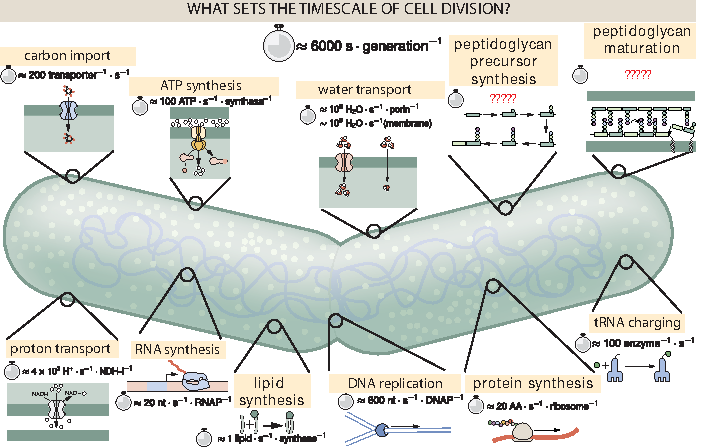
\includegraphics{../../figures/categories.pdf}
    \caption{\textbf{Transport and synthesis processes necessary for cell division.}}
    \label{fig:categories}
    }
\end{figure}



Points to emphasize
\begin{itemize}
\item The past decade of work in proteomics has made high-througput absolute
measurement of protein abundance a reality. Recent groups have used mass
spectrometry and ribosomal profiling to quantify growth-dependent effects on
protein copy numbers across growth conditions. In this work, we assemble four
recent datasets that examine how cellular proteome is influenced by the total
growth rate. 
\end{itemize}
\section{A comprehensive examination of the \textit{E. coli} proteome}


\begin{figure}
{  \centering 
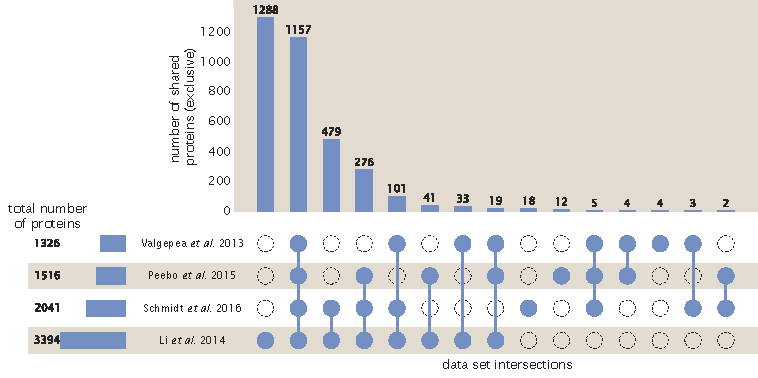
\includegraphics{../../figures/dataset_upset_diagram.pdf}
\caption{\textbf{Summary of the compiled datasets.}}

}
\label{fig:datset_intersections}
\end{figure}



\begin{figure}
    \centering{
        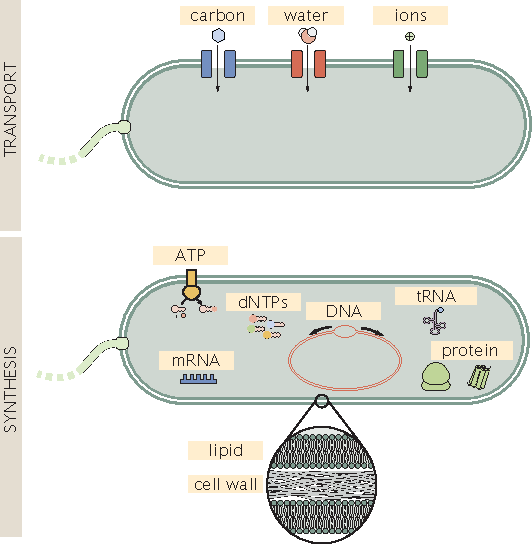
\includegraphics{../../figures/estimation_categories.pdf}
        \caption{\textbf{Potential bottlenecks for bacterial growth.} The
        growth rate of \textit{Escherichia coli} may be limited by the
        transport of biochemical precursors across the cell membrane (top
        panel) or by the synthesis of various molecules and macromolecules.
        Illustrative examples of the potential bottlenecks are provided in
        both panels.}        
    \label{fig:categories}
    }
    \end{figure}
    
\section{Transport of Biochemical Building Blocks}
We begin with an interrogation of some of the myriad transport systems bacteria
use to bring extracellular materials (such as carbon, water, and ions) into the
cell. 

\subsection{Carbon Transport}
All macromolecules synthesized by cells include carbon as the primary elemental 
constituent. It is therefore reasonable to consider the acquisition of carbon
from the environment, typically in the form of sugar, as a candidate process 
which sets the bacterial speed limit. We can a combination of biological intuition
and the vast literature on the molecular composition of \textit{E. coli} to make 
an order-of-magnitude estimate for the total number of sugar transporters needed 
double. 

For convenience, we will consider a condition in which glucose is the primary
carbon source in a growth medium. In standard laboratory conditions, a
minimal medium supplemented with only glucose will have a growth rate of
$\approx 1 \text{generation}\cdot\text{hr}^{-1}$ which is an approximate
doubling time of $\approx 3000 $ seconds. During this time, the cell must be
able to import enough carbon molecules to double all macromolecules.  

We can begin by using the well justified estimate that the typical \textit{E. coli}
cell is $\approx$ 70\% water by mass, yielding a $\approx$ 30\% dry mass (BNID: 109049, \cite{milo2010}).
Exponential growth of \textit{E. coli} in a glucose based medium results in an 
average cell volume of 1 fL, bringing our total dry mass to 30 pg. Assuming half of 
this dry mass is protein (0.15 pg), we can estimate how many carbons are present in 
the protein pool.   

Let's assume that a standard protein is approximately 300 amino acids long,
which comes out a mass of $\approx$ 30 kDa. From this, we estimate that the
total number of amino acids (incorporated into protein) is
\begin{equation}
    N_\text{AA} = \left(1.5 \times 10^{-13}\,\text{g}\right) \times
\left({1\,\text{protein} \over 3 \times 10^4\, \text{Da}}\right) \times
\left( {6 \times 10^{23}\,\text{Da} \over 1\,\text{g}}\right) \times \left({3
\times 10^2 \,\text{AA} \over \text{protein}}\right) \approx 2.5 \times
10^8\,\text{Amino\, Acids}. 
\label{eq:num_amino_acids}
\end{equation}
The typical amino acid consists of a two-carbon backbone with a $\approx$ 3
carbon side-chain. Thus, assuming the typical amino acid contains $\approx$ 5
carbons, the total mass of carbon in the protein pool can be calculated as
\begin{equation}
    N_\text{C}^\text{(protein)} = N_\text{AA} \times {\text{C} \over \text{AA}}
= 2.5 \times 10^8\, \text{AA} \times {5\, \text{C} \over \text{AA}} \approx 5
\times 10^9\, {\text{C} \over \text{cell}}. 
\label{eq:n_carbon_protein}
\end{equation}
Since we approximated that about half of the dry mass is protein, it's
reasonable to assume that the remaining half of the dry mass has a similar
composition, permitting us to say that
\begin{equation}
N_\text{C}^{\text{(cell)}} \approx 2 \times N_\text{C}^\text{(protein)} =
10^{10} {\text{C} \over \text{cell}}. 
\label{eq:n_carbon_cell}
\end{equation}
With a handle on the total number of carbons needed per cell, we can now try
to estimate how many sugar transporters would be needed to transport 100
billion carbon atoms per standard cell doubling time of $\approx 3000$ seconds. With 6
carbon atoms per glucose molecule, we can estimate the minimum glucose flux
across the membrane to be
\begin{equation}
J_\text{glucose} = {10^{10}\,\text{C} \over \text{cell}} \times {1\,
\text{glucose} \over 6\, \text{C}} \times {1\,\text{cell} \over 3 \times
10^3\,\text{s}} \approx 5 \times 10^6 {\text{glucose} \over \text{s}}.
\label{eq:glucose_flux}
\end{equation}
The chief glucose transport system of \textit{E. coli} (the PTS system) can 
transport $\approx 200\, \text{glucose}\cdot\text{s}^{-1}$ (BNID: 103693 \cite{milo2010})
meaning that the \textit{minimum} number of glucose transporters per cell needed 
to double the cellular carbon content is
\begin{equation}
N_\text{tpr.} \approx {J_\text{glucose} \over J_\text{transporter}} = {5
\times 10^6 \text{glucose / s} \over 2 \times 10^2 \,\text{glucose / s}}
\approx 2 \times 10^4\, \text{tpr. / cell}.
\label{eq:n_gluc_transporters}
\end{equation}




\subsection{Water Transport}

\bibliography{library.bib}
\end{document}